\documentclass{article}

%Headers
\usepackage[dvips]{graphicx}    %package that does pdfs
\usepackage{color}              %this needs to be here also

\title{CS440: The Maze is on Fire}
\author{Andy Rivera, John Juarez}
\date{February 19, 2021}

\begin{document}
\maketitle

\section{Maze Generation and Project Setup}
   To generate a maze we used the function \textbf{generateMaze(int dim,double p)} it takes in the parameters of  \textit{dim} to construct a dimxdim 2D array and \textit{p} to determine the probability of a block being filled(1) or not(0).
   
   To set up the project for the path finding algorithms we created an object \textbf{Point} with the following attributes:
   \begin{itemize}
   \item Point parent (Previous location of agent)
   \item X and Y to keep track of location of agent
   \item stepsTaken (Amount of steps taken to get to the current location.)
   \item Hueristics (Estimate for A* algorithm)
   \end{itemize}

\begin{figure}[hpt]

\centering
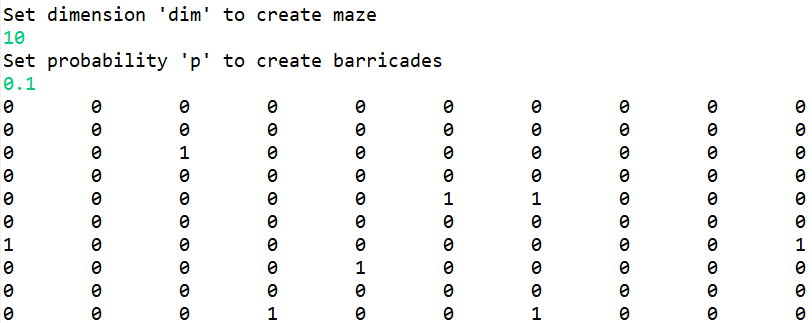
\includegraphics[width=3.2in]{maze1}\hfill
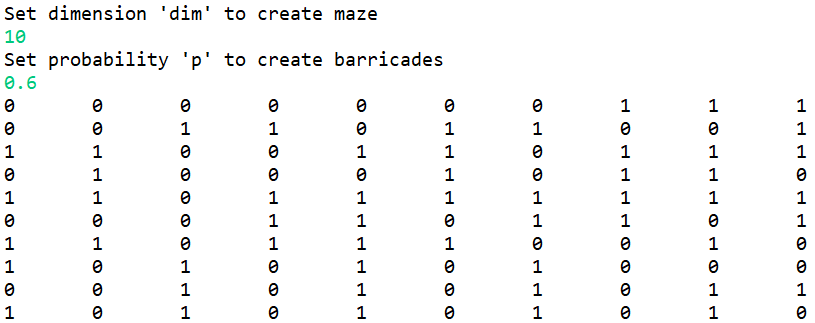
\includegraphics[width=3.2in]{maze3}

\caption{Maps generated with p = 0.1 and 0.6 respectively}
\label{fig:figure1}

\end{figure}

\section{DFS Algorithm}
 We created the method \textbf{mazeDFS(int[][] maze, Point start, Point goal).} It takes in 2 points and returns a boolean, True if there exists a path and false if no path exists between the starting point and the goal point. 
	
	With two arbitrary points in the maze, DFS would be a better option because we are just determining if there is a path between the two points and not necessarily the shortest path, it will save space in memory since it adds less points into the fringe by not exploring all of its neighbors.
	\begin{figure}[hpt]

\centering
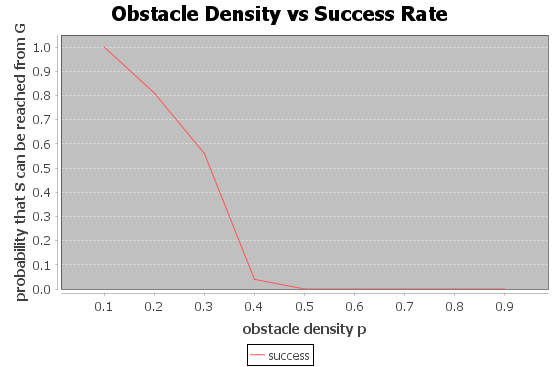
\includegraphics[width=3.2in]{DFSanalysis}

\caption{obstacle density p vs probability that S can be reached from G}
\label{fig:figure2}

\end{figure}

\section{BFS and A* Algorithms}
  For our BFS algorithm, we created the method mazeBFS(int[][] maze). It returns an ArrayList of points that create a minimal path that exists from the start to goal state. In order to avoid an endless traversal of the same path, another ArrayList is used to keep track of the Points that have already been explored.
   
For our A* algorithm, we created the method mazeAStar(int[][] maze). It uses a priority queue that prioritizes points based on the heuristic. The heuristic for a point is determined by a 3-step formula, de-prioritization of paths that take steps backwards, i.e. ‘left’ and ‘up’, prioritization of paths closer to the goal state, and extra priority for the paths that have open space in either forward direction, i.e. ‘right’ and ‘down’. Essentially, the idea behind the algorithm was to focus on paths with the most open space up ahead that can take the agent the furthest, closer to the goal, and provide much more alternatives in the case of an obstructed path. If the path is obstructed and the only possible movement is a backward step, the algorithm will then opt for an earlier point in the path that is still relatively close to the goal state and has plenty of open space ahead of it for exploration.
   
   If there is no path between the starting point and the goal point the difference between nodes explored by BFS and A* would be 0 because both algorithms would keep trying to explore every point in the maze.                                                     
   
   \begin{figure}[hpt]
   \centering
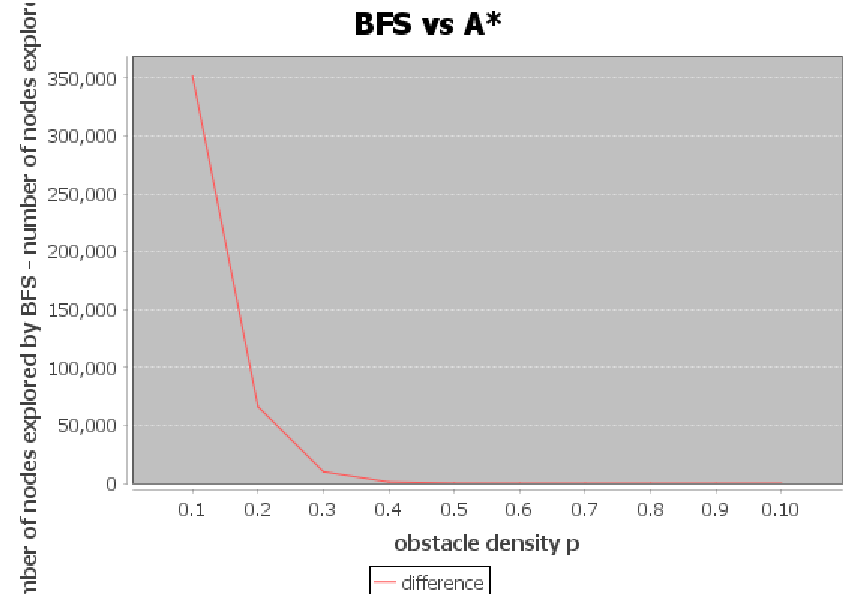
\includegraphics[width=3.2in]{BFSvA}

\caption{number of nodes explored by BFS - number of nodes explored by A* vs obstacle density p}
\label{fig:figure3}

\end{figure}
   
   \begin{figure}[hpt]
   \centering
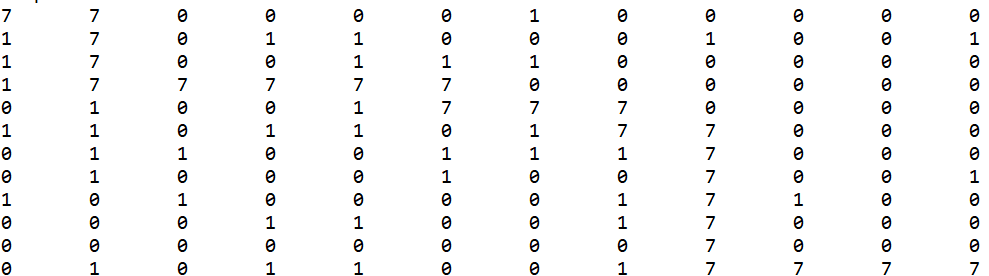
\includegraphics[width=3.2in]{BFS}

\caption{BFS Shortest path represented by 7 dim = 12 p = 0.3}
\label{fig:figure4}

\end{figure}

 \begin{figure}[hpt]
   \centering
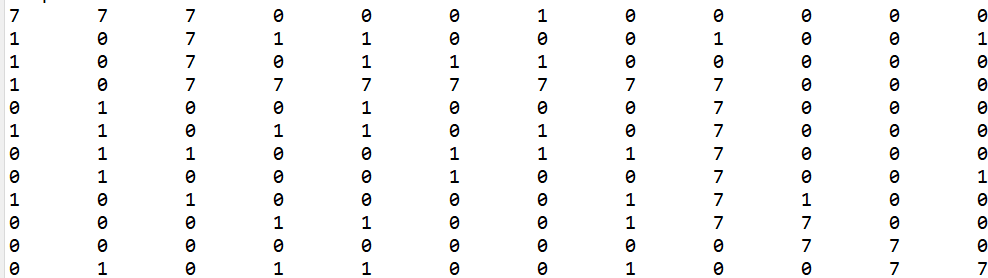
\includegraphics[width=3.2in]{astar}

\caption{A* Shortest path represented by 7 dim = 12 p = 0.3}
\label{fig:figure5}

\end{figure}
\bigskip
\bigskip


\section{Algorithms in less than 1 minute}	
At p = 0.3 the largest dimension size the algorithm can find a path in less than one minute is...
\begin{itemize}
\item \textbf{DFS} dim = 500
\item \textbf{BFS} dim =
\item \textbf{A*}  dim =
\end{itemize}

\section{Strategy 3}
For our implementation of Strategy 3, we took an approach that would only re-compute a new path when a point in the path is on fire or if a point in the path is at risk of being on fire soon. Upon each step, our algorithm scans the maze and keeps track of all the points that are currently on fire. It then scans the path ahead of the agent’s position and considers how the fire will look in the future by taking an estimate of the steps needed for the fire to reach a point in the path by counting the cells in between each fire point and path point. If a fire point is less than 4 steps away from a point in the path, we consider that point to be at risk, and so we compare the current position of that agent relative to that point at risk and see if the agent will pass that point prior to the fire ever being able to obstruct it. 
	
	If so, then nothing needs to be done since the agent will pass the point safely, otherwise, we determine the accurate amount steps from the fire to the point at risk by running a modified Breath-First Search algorithm. This modified BFS algorithm will either return null in the case of: no path exists from the fire point to the risk point, the algorithm is running too long (likely due to a long path that exceeds 3 steps), or the accurate amount of steps is more than the amount of steps the agent needs to pass the point. In the case that the algorithm does return a path from the fire point to the path point at risk, this path of fire will be simulated in a temporary copy of the maze where the algorithm will attempt to create a new path using the A* algorithm that avoids the simulated path of fire, if possible, otherwise, the agent will have to take the risk and traverse the same path.  
   
   \begin{figure}[hpt]
   \centering
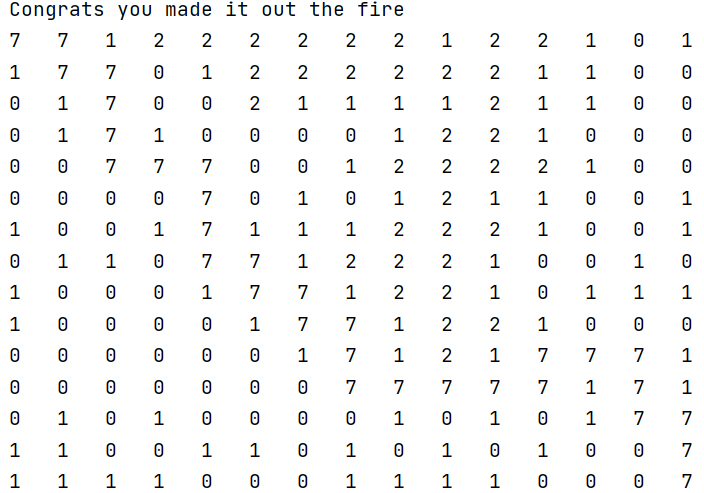
\includegraphics[width=3.5in]{strat3ex}

\caption{Strategy 3: dim = 15, p=0.3, q=0.3
7-represents path 2-represents fire}
\label{fig:figure6}
\end{figure}

\bigskip
\bigskip
\bigskip
\bigskip
\bigskip
\bigskip
\bigskip
\bigskip

\section{Strategies Success Rates}
At a low probability q the strategies are performing performing similarly at high success rates. As the fire starts spreading faster through the maze the success rates decrease. Between q values of 0.3-0.7, strategy 3 performs 10% better since it tries to predict the path of the fire as well. 
  
\begin{figure}[hbt!]
   \centering
\includegraphics[width=3.5in]{stratAnalysis}

\caption{Strategies Analysis created for mazes with dim size 50 and p =0.3}
\label{fig:figure7}
\end{figure}

\begin{figure}[hbt!]
   \centering
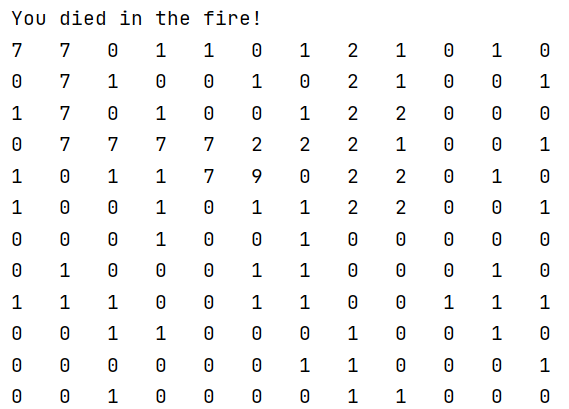
\includegraphics[width=3.5in]{strat1fail}

\caption{Strategy 1 failed attempt at dim = 12, p=0.3 q=0.3 7-represents path 9-represents agent catching on fire 2-represents fire}
\label{fig:figure8}
\end{figure}

\begin{figure}[hbt!]
   \centering
\includegraphics[width=3.5in]{strat2Success}

\caption{Strategy 2 Success at dim = 15, p=0.3 q=0.3 7 represents path 2-represents fire}
\label{fig:figure9}
\end{figure}


\section{Unlimited Computational Resources}
If we had unlimited computational resources, we would likely look to improve strategy 3 by adding an extra level of estimation of probability before resorting to finding new paths that avoid risky points. Essentially, we would change our Strategy 3 by getting an accurate number of steps from each fire point to each path point using our modified BFS algorithm right away, rather than counting the cells in-between as an estimate. We would then be able to calculate an accurate probability for each path point being set on fire: $q^{k} (k = number of steps in the fire path)$ while also considering adjacent fire neighbors that would increase the likelihood of points in the fire path being set on fire, further increasing the probability of flammability for the path point. We would only consider the probabilities with the least amount of steps to the path point. If the probability of flammability is above a certain threshold, we then count the steps before the agent passes this point at risk, if it’s more than the amount of steps before the fire reaches the path point, we will then opt for a new path by simulating this fire path and avoiding it if possible.

 This would improve strategy 3 by resulting in less unnecessary re-computations of paths. Rather than re-computing simply based on the number of steps in between the fire point and path point, it will also consider the probability of that path point being set on fire in x amount of steps. Re-computing less unnecessary paths also means a lower likelihood of having to take backward steps to avoid the ‘possible’ fire and reaching the goal state much quicker.

\section{10 Seconds to Make a Move}
	If we had 10 seconds between moves, our algorithm of scanning the path and generating a new path at every move would work within those 10 seconds.  Since DFS is more less computational that both BFS and A*, it will be more efficient to through that route and instead of adding points into the fringe, we can incorporate heuristics. We can calculate the euclidean distance from the agent to the closest location of the fire and the euclidean distance from the goal. Maximum distance from fire + minimum distance from fire. It will choose its next block greedily since it it is only looking at it's neighbors.  
\end{document}
